\documentclass[11pt,a4paper,titlepage, ngerman]{article}

\usepackage[utf8]{inputenc}	
\usepackage[T1]{fontenc}	
\usepackage{ngerman}			
\usepackage{lmodern}			
\usepackage{graphicx}			
\usepackage{url}				
\usepackage{siunitx}
\usepackage[intlimits]{amsmath}
\usepackage{xfrac}
\usepackage{commath}
\usepackage{physics}			
\usepackage{subcaption}
\usepackage{wrapfig}
\usepackage{biblatex}
\usepackage{hyperref}
\usepackage{textcomp}

% Setup SI unit environment
\sisetup{separate-uncertainty = true}
\sisetup{output-decimal-marker = {,}}
\sisetup{
	per-mode=fraction,
	fraction-function=\sfrac
	% or \frac, \tfrac
}
\bibliography{Literatur}

\begin{document}
	\begin{titlepage}
		\centering
		{\scshape\LARGE Versuchsbericht zu \par}
		\vspace{1cm}
		{\scshape\huge M5 -- Jo-Jo und Kreisel\par}
		\vspace{2.5cm}
		{\LARGE Gruppe 10 Mi\par}
		\vspace{0.5cm}
		{\large Alex Oster (E-Mail: a\_oste16@uni--muenster.de) \par}
		{\large Jonathan Sigrist (E-Mail: j\_sigr01@uni--muenster.de) \par}
		\vfill
		durchgeführt am 21.12.2017\par
		betreut von\par
		{\large Lukas \textsc{Britt}} 
		\vfill	
		{\large \today\par}
	\end{titlepage}
	
	\tableofcontents
	
	\newpage
	
	\section{Kurzfassung}
	
	% Einleitung & Beschreibung der Versuche
	
	Dieser Bericht beschäftigt sich mit der Untersuchung der Trägheit. Dazu werden zwei Versuche herangeführt, welche diese auf verschiedene Weisen darstellen.
	
	Der erste Versuch zu dem Fallrad zeigt ein Verhalten, welches einem Jo-Jo ähnelt. Ein langsames Abrollen und darauffolgendes Aufrollen. Hierbei wird jedoch das Abrollen genauer betrachtet. Es werden die Fallbeschleunigung und das Trägheitsmoment bestimmt und mit theoretischen Zusammenhängen, wie z. B. mit dem Abrollradius in Verbindung gebracht und die Theorie mit übereinstimmenden Werten bestätigt.
	
	Der zweite Versuch zeigt, dass ein Kugelkreisel durch seine Trägheit im rotierenden Zustand eine gleichförmige Bewegung durchführt.
	Es tritt eine Präzessionsbewegung auf, mit welcher sich die Figurenachse des Kreisels langsam aber gleichmäßig um die Senkrechte dreht.
	Durch die Präzessionseffekte wird das Trägheitsmoment bestimmt und mit weiteren theoretischen Werten verglichen.
			
	\vspace{2cm} 
	
	\section{Fallrad} % vorläufiger Name
	
	Das Fallrad verhält sich wie das Jo-Jo Spielzeug. Lässt man das aufgewickelte Fallrad fallen, bei festgehaltener Schnur, so fällt es langsamer und und wickelt sich nach Abwickeln der Schnur von selbst wieder auf. In diesem Versuch werden die Fallbeschleunigung und das Trägheitsmoment eines Fallrades bestimmt und überprüft, ob die gemessenen und bestimmten Werte mit den aus der Theorie berechneten Werten übereinstimmen. Dazu wird angenommen, dass die aus der Theorie bekannten Formeln den Sachverhalt korrekt beschreiben. Das Ergebnis dieses Versuches stimmt mit diesen (nicht) überein. % TODO 
	
	\subsection{Methoden}
		
		\subsubsection{Aufbau}
		
			\begin{figure}[ht]
				\centering
				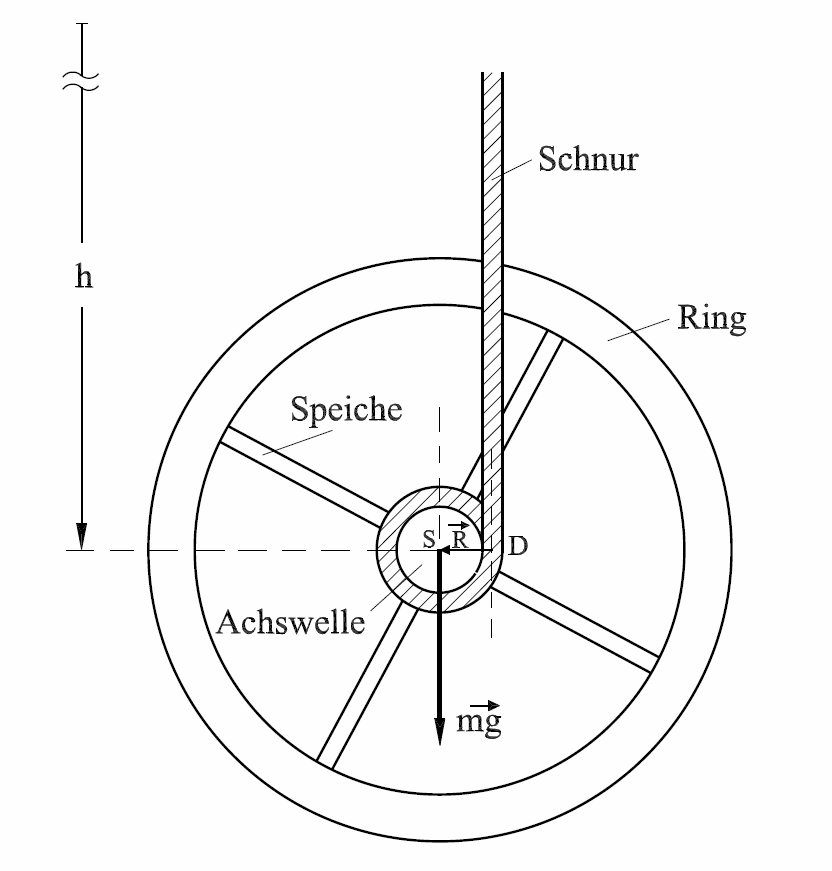
\includegraphics[width=0.7\textwidth]{fallrad_skizze.png}
				\caption{Versuchsskizze: Seitenansicht des Fallrades}
				\label{fig:FallradSkizze}	
			\end{figure}
			Es wird der in Abb. \ref{fig:FallradSkizze} dargestellte Aufbau betrachtet. 
			Das Fallrad besteht aus einem Ring, in dessen Mittelpunkt sich die Achse befindet, um welche die Bewegung durchgeführt wird. Mit Hilfe von vier Speichen ist der Ring mit der Achse verbunden. Zur Vereinfachung wird angenommen, dass es sich hierbei um zwei senkrecht zueinander liegende Zylinder handelt, die in ihren Mittelpunkten mit der Achse verbunden sind. 
			Die Achse liegt mittig in dem Ring, sodass die Schnur auf beiden Seiten mit dem gleichen Abstand von dem Ring angebracht werden kann (vgl. \ref{fig:FallradFrontal}). 
			\begin{figure}[ht]
				\centering
				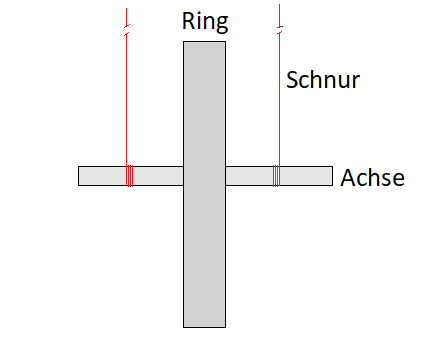
\includegraphics[width=0.6\textwidth]{fallrad_frontal.png}
				\caption{Frontalansicht des Fallrades}
				\label{fig:FallradFrontal}	
			\end{figure}
			In der Ruhelage liegen keine Wicklungen der Schnur auf der Achse vor. Die Größe $h$ gibt die Höhe des Fallrades, als Abstand von der Ruhelage, an. 
		
		\subsubsection{Durchführung}
			
			Mit einer Stoppuhr wird die Zeit gemessen, die das Fallrad benötigt bis keine Wicklung des Fadens auf der Achse vorliegt. Dies wird für verschiedene Starthöhen durchgeführt um die Fallbeschleunigung $g^{*}$ zu bestimmen. Dafür ist es wichtig darauf zu achten, dass die Schnur sich bei dem Aufwickeln nicht auf sich selber, sondern nur auf der Achse wickelt, damit sich der Abrollradius nicht verändert.
			Die Höhe wird von einem Maß abgelesen, wobei das Fallrad in Ruhelage (bzw. wenn keine Wicklung des Fadens auf der Achse vorliegt) bei genau \SI{0}{\cm} an dem Maß liegt. 
			
			Zur Bestimmung des Trägheitsmoments werden die Maße des Fallrads mit Hilfe einer Schiebelehre gemessen und die Masse gewägt.			
			
		\subsubsection{Unsicherheiten}
			
			Im Allgemeinen dient zur Berechnung der Unsicherheiten für die gemessenen und ermittelten Werte folgende Formel: 
			\begin{equation*}
				u(s) = \pm \sqrt{\sum_{k=0}^{N}\left( \frac{\partial f}{\partial x_i}u(x_i)\right) ^2}. \label{eq:kombUnsicherheit}
			\end{equation*}
			Für die Messunsicherheit der Stoppuhr wird aufgrund der Digitalanzeige eine Rechtecksverteilung verwendet und diese dann mit der Unsicherheit für die Reaktionszeit\footnote{hierzu werden \SI{0.1}{\s} dreiecksverteilt verwendet} kombiniert. Die Schiebelehre besitzt eine Messgenauigkeit von \SI{0,02}{\mm}, da sich so genau jedoch nicht ablesen lässt, wird eine Dreicksverteilung über \SI{0,04}{\mm} verwendet. Für das Maß wird ebenfalls eine Dreiecksverteilung gewählt, hierbei über \SI{1}{\mm}.
			Die Berechnung der Unsicherheiten liegt im Anhang (\ref{Anhang})  vor, da diese für einige Größen umfangreicher ist.
			
	\subsection{Messung}
	
		\subsubsection{Messwerte}
			
			Die in Tab. \ref{tab:Messwerte} dargestellten Werte sind die (gemittelten) Messwerte, welche aufgenommen wurden. Dabei ist die Berechnung der verwendeten kombinierten Unsicherheiten, für z. B. die gemittelten Werte, dem Anhang zu entnehmen.
			\begin{table}[ht]
				\caption{In dieser Tabelle sind die gemessenen Werte verzeichnet. Die Größen welche mehrmals gemessen wurden, sind hier gemittelt.}
				\centering
				\label{tab:Messwerte}
				\begin{tabular}{l c}
					{Maße des Fallrads} &
					\begin{tabular}{l l}
						\begin{tabular}{l|l}
							{Größe} & {Wert}	\\
							\hline
							{Dicke $H$ des Rings} & {\SI{11,68+-0,03}{\mm}} \\
							{Außenradius $R_a$ des Rings} & {\SI{90,08+-0,01}{\mm}} \\
							{Innenradius $R_i$  des Rings} & {\SI{77,59+-0,01}{\mm}} \\
							{Speichenradius $R_S$} & {\SI{3,490+-0,006}{\mm}} \\
							{Achsenradius $R_A$} & {\SI{4,090+-0,006}{\mm}} \\
							{Achsenlänge $L_A$} & {\SI{200,3+-0,002}{\mm}} \\
							{Masse $m$} & {\SI{768,16+-0,01}{\g}} \\
							{Fadendicke $d$} & {\SI{1,027+-0,028}{\mm}} \\
						\end{tabular}	
					\end{tabular}
					\\ & \\
					{Fallhöhe und Fallzeit} &
					\begin{tabular}{l|l}
						{Fallhöhe $h$} & {Fallzeit $t$}	\\
						\hline
						{\SI{200+-0,29}{\mm}} & {\SI{3,402+-0,046}{\s}} \\
						{\SI{350+-0,29}{\mm}} & {\SI{4,488+-0,046}{\s}} \\
						{\SI{500+-0,29}{\mm}} & {\SI{5,286+-0,046}{\s}} \\
						{\SI{650+-0,29}{\mm}} & {\SI{6,122+-0,046}{\s}} \\
						{\SI{800+-0,29}{\mm}} & {\SI{6,782+-0,046}{\s}} \\
					\end{tabular}
				\end{tabular}					
			\end{table}
			
		\subsubsection{Messergebnisse}	
			
			\begin{figure}[ht]
				\centering
				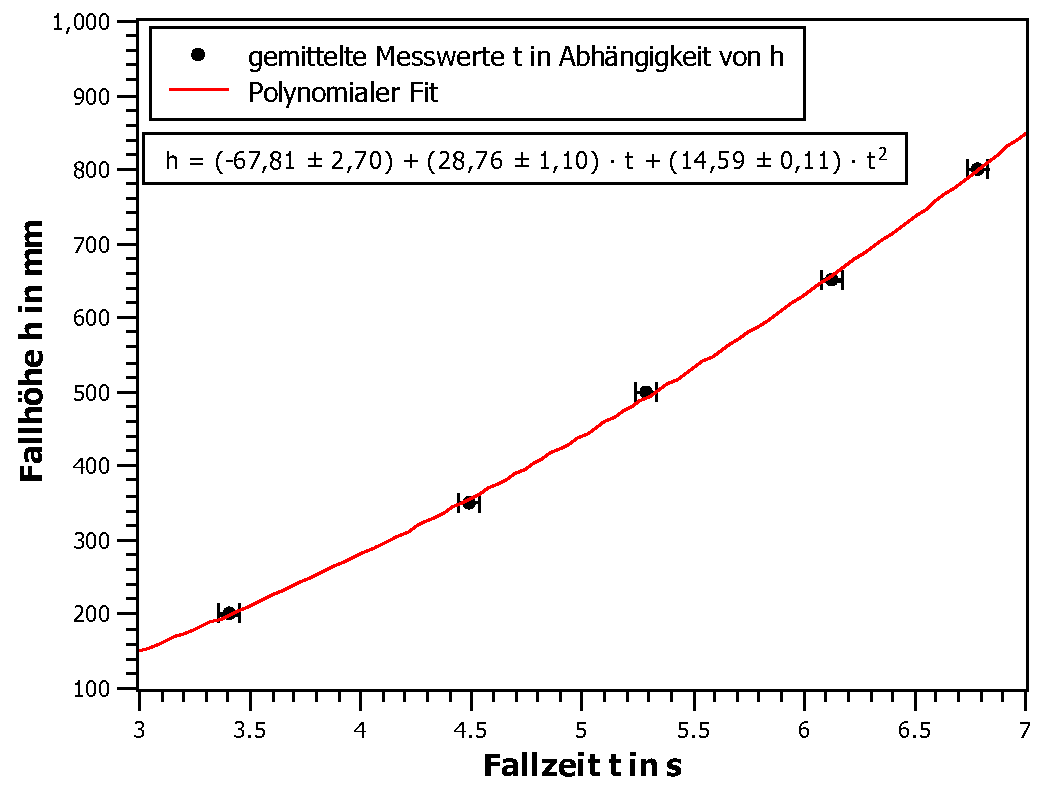
\includegraphics[width=\textwidth]{h-gegen-t.pdf}
				\caption{Graphische Darstellung der Fallhöhe $h$ in Abhängigkeit der Fallzeit $t$.}
				\label{fig:hgegent}	
			\end{figure}
			In dem Ersten der drei folgenden Diagrammen (Abb. \ref{fig:hgegent}) ist die Fallhöhe $h$ gegen die Fallzeit $t$ aufgetragen.
			Aufgrund des leicht gekrümmten Verlaufs und der Formel zur Berechnung der Fallhöhe
			\begin{equation}
				h(t) = \frac{1}{2}g \frac{mR^2}{J_S + mR^2} t^2 = \frac{1}{2}g^{*}t^2 \label{eq:Fallbeschleunigung}
			\end{equation}
			wurde ein polynomialer Fit\footnote{Dieser Fit und seine Unsicherheit, wie auch die der nächsten beiden, wurde von dem Programm SciDavis berechnet, dazu wurden die Unsicherheiten (welche im Anhang zu finden sind) und die Methode der kleinsten Quadrate herangezogen} für das Diagramm gewählt.
			Der Fit besitzt folgende Form: 
			\begin{equation*}
				h(t) = [(-67,81\pm 2,70)+(28,76\pm 1,10)t\cdot\si{s^{-1}}+(14,59\pm 0,11)t^2\cdot\si{s^{-2}}]\si{\mm}.
			\end{equation*} 
			\begin{figure}[ht]
				\centering
				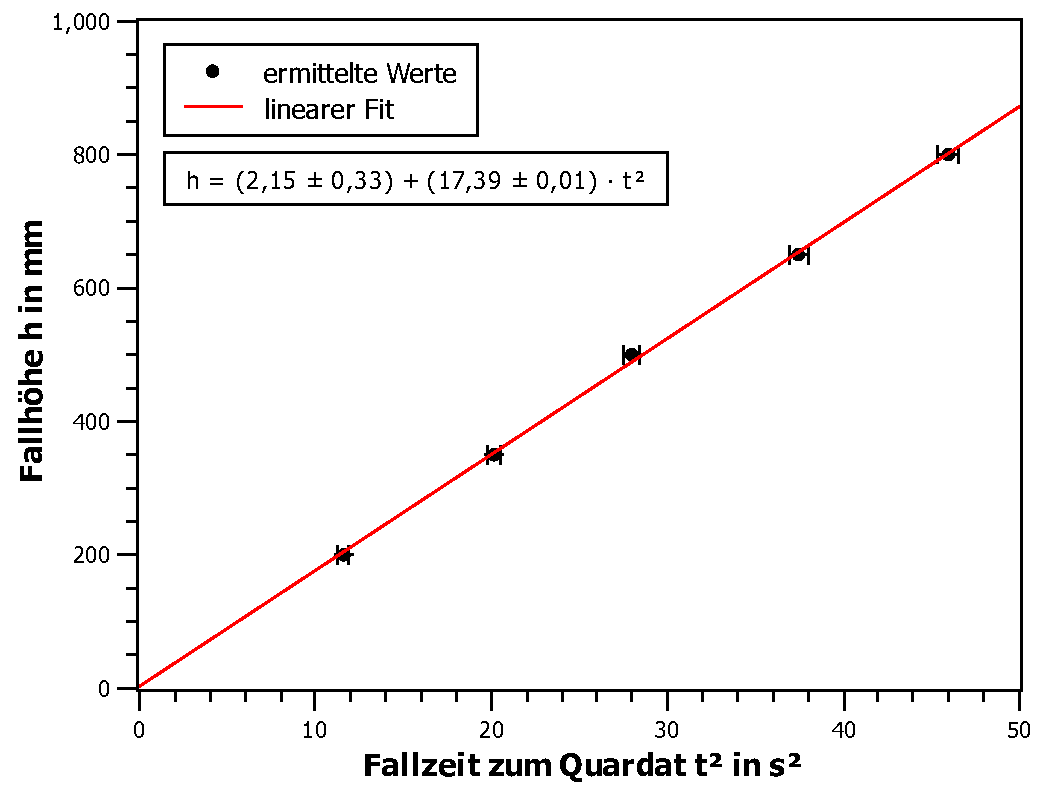
\includegraphics[width=\textwidth]{h-gegen-t2.pdf}
				\caption{Graphische Darstellung der Fallhöhe $h$ in Abhängigkeit der Fallzeit $t$.}
				\label{fig:hgegent2}	
			\end{figure}	
			Da im zweiten Diagramm die Fallhöhe $h$ gegen die quadrierte Fallzeit $t^2$ aufgetragen ist, sollte sich hierbei nach obiger Gleichung ein linearer Zusammenhang zeigen. Aus diesem Grund wurde für dieses Diagramm ein linearer Fit gewählt. Hierbei sollte die Steigung nach Gl. \ref{eq:Fallbeschleunigung} gerade gleich der halben Fallbeschleunigung $g^{*}$ entsprechen. Folgende Formel beschreibt den Fit:
			\begin{equation*}
				h(t) = [(2,15 \pm 0,33)+(17,39 \pm 0,01)t^2\cdot\si{s^{-2}}]\si{\mm}.
			\end{equation*} 
			\begin{figure}[ht]
				\centering
				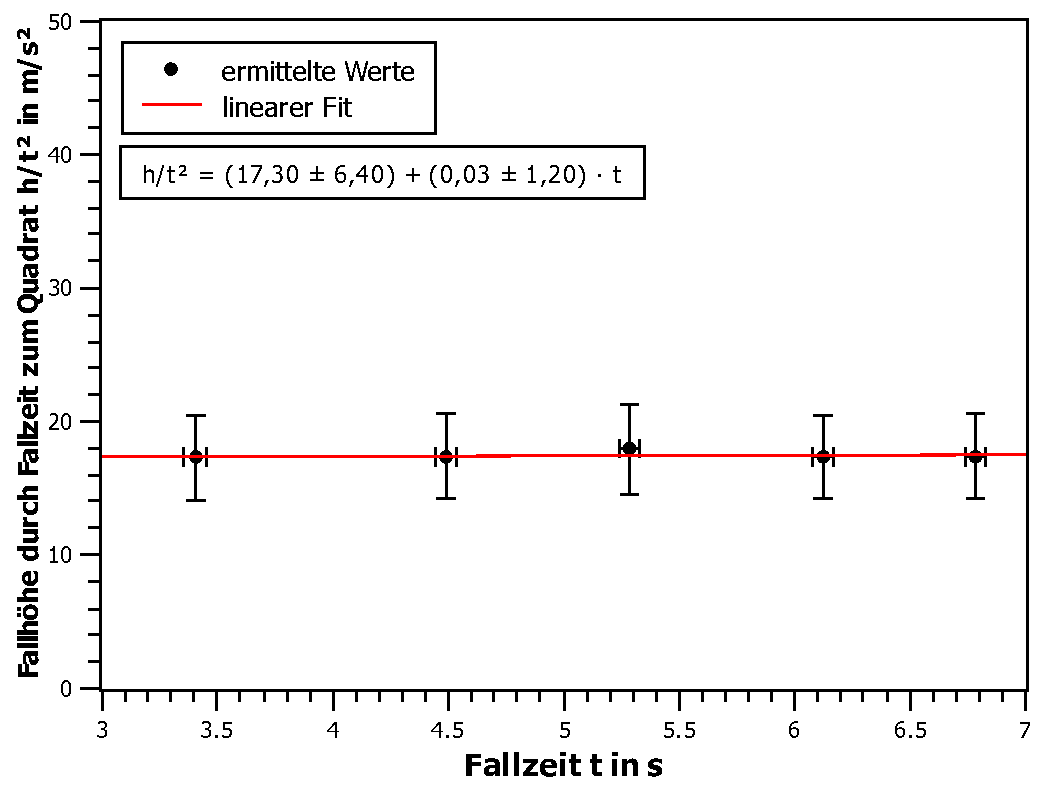
\includegraphics[width=\textwidth]{ht2-gegen-t.pdf}
				\caption{Graphische Darstellung der Fallhöhe $h$ in Abhängigkeit der Fallzeit $t$.}
				\label{fig:ht2gegent}	
			\end{figure}
			Da diese Steigung nicht von der Zeit abhängt, ist wie in dem letzten Diagramm näherungsweise zu sehen $\frac{h}{t^2}$ konstant. Auch hier wurde aufgrund dieses Verhaltens ein linearer Fit gewählt. Da die ermittelten Punkte auf einer Horizontalen liegen zu scheinen ist die Steigung demnach $\approx 0$. Aufgrund der Unsicherheit, welche merklich von null entfernt ist, wird dies jedoch nicht ganz gestützt. Der Fit sieht wie folgt aus:
			\begin{equation*}
				\frac{h}{t^2} = [(17,30 \pm 6,40) + (0,03 \pm 1,20)t\cdot\si{s^{-1}}]\si{\mm}.
			\end{equation*} 
			Wählt man die Steigung gleich null und multipliziert man das Ergebnis mit zwei, so ergibt sich für $g^{*} = \SI{34,6+-12,8}{\m\per\s^2}$. 
					
			Zur Bestimmung des Trägheitsmoments $J_S$ des Fallrads werden die Trägheitsmomente der Bestandteile addiert. Diese lassen sich durch Zylinderträgheitsmomente bestimmen. Für den Ring wird die Formel für einen Hohlzylinder verwendet, welcher parallel zur Drehachse liegt:
			\begin{align}
					J_{parallel} = \frac{1}{2}\pi H\rho(R_a^4-R_i^4). \label{eq:Trägpar}
			\end{align}
			Ebenso lässt sich das Trägheitsmoment der Achse bestimmen, da es sich hierbei jedoch um einen Vollzylinder handelt wird der Innenradius in der Formel gleich null gesetzt.
			Für die vier Speichen wird vereinfacht, so dass nur zwei Zylinder senkrecht zur Drehachse betrachtet werden.
			Dieses bestimmt sich wie folgt: 
			\begin{align}
				J_{senkrecht} = \pi H\rho\left[\frac{1}{12}H^2R^2+\frac{1}{4}R^4\right]. \label{eq:Trägsenk}
			\end{align} 
			Zur Bestimmung der Dichte muss das Volumen bestimmt werden und die gemessene Masse dadurch geteilt werden. Das Volumen setzt sich wie auch das Trägheitsmomenten aus den Einzelteilen zusammen:
			\begin{equation}
				V = V_{Ring} + 2\cdot V_{Speiche} + V_{Achse} = H\cdot(\pi R_a^2 - \pi R_i^2) + 2(2\pi R_S\cdot 2 R_i) + 2\pi R_A\cdot L_A.
			\end{equation}
			Dabei bezeichnet $V_{Speiche}$ das Volumen von zwei der vier Speichen, welches durch einen Zylinder mit Radius $R_S$ und Höhe $R_i$ zusammengesetzt ist. Dies ist eine Näherung da hierbei das Volumen im Mittelpunkt des Fallrades drei mal, durch die zwei Speichenzylinder und die Achse, in der Rechnung auftaucht, jedoch auch das Volumen des Befestigungspunktes dieser Teile vernachlässigt wird.
			Mit der Masse $m=$ und dem Volumen $V=$ ergibt sich eine Dichte $\rho = $. Auch hier wurden die verwendeten Unsicherheiten in dem Anhang hergeleitet.
			Durch die Summe der Trägheitsmomente ergibt sich somit:
			\begin{equation}
				J_S = J_{Ring} + 2\cdot J_{Speiche} + J_{Achse} = = %Erg.
			\end{equation}
			
			Aus dem ermittelten Trägheitsmoment und der Fallbeschleunigung lässt sich nun der Abrollradius durch Umformen von Gl. \ref{eq:Fallbeschleunigung} bestimmen.
			\begin{equation}
				R = \sqrt{\frac{J_S \cdot g^{*}}{m(g-g^{*})}} = %erg.
			\end{equation}
			Durch den Radius der Achse und dem des Fadens ergibt sich für den Abrollradius $R = \SI{4,604+-0,015}{\mm}$.
			
	\subsection{Diskussion}
		
		
		
	\subsection{Schlussfolgerung}
	 
	\newpage
	\section{Kreisel} % vorläufiger Name

In dem zweiten Teilversuch  soll das Trägheitsmoment eines schweren, symmetrischen Kreisels bestimmt werden.
Dazu wird es zuerst direkt durch die geometrische Form berechnet und dann mit Hilfe der Präzession graphisch ermittelt.

\subsection{Methoden}

	\subsubsection{Aufbau}
	
	Ein Kreisel besteht aus einer Metallkugel, einer Verbindungsstange und einem an dieser verschiebbaren Gewicht.
	Der Kreisel wird auf ein Luftkissen annähernd reibungsfrei gelagert.
	Zudem wird so der Unterstützungspunkt im Kugelmittelpunkt gehalten.
	Zunächst stehe der Kreisel aufrecht.
	Die Kugel wird nun tangential mit Druckluft angeblasen, bis der Kreisel stabil rotiert.
	Der Kreisel wird in etwa um den Winkel $\frac{\pi}{4}$ gekippt und präzessiert nun zusätzlich um die Senkrechte.
	Für eine weitere Stabilisierung kann der Kreisel einmal am Finger entlang geleitet werden, um unregelmäßige Bewegungen weitgehend zu vermeiden.
	
	Ein Stroboskoplicht wird eingeschaltet und auf eine bestimmte Frequenz eingestellt.
	Durch einen kleinen weißen Punkt auf der Kugel kann die Rotation des Kreisels mit der Frequenz des Stroboskoplichtes synchronisiert werden.
	Dies ist dann erreicht, wenn sich der Punkt scheinbar nicht mehr bewegt.
	Dabei kann eine feine Abstimmung durch Variation des Abstandes und des Winkels der Druckluftdüse zu der Metallkugel erreicht werden.
	
	\subsubsection{Komplikationen}
	
	Der erste verwendete Kreisel war nicht ganz stabil und die Präzessionsbewegung wies stets nach kurzer Zeit unruhige Bewegungen auf.
	Das kommt wahrscheinlich von einer Unwucht, also einer Deformation des Kreisels.
	
	Der Kreisel ist beim Abbremsen von einer hohen Frequenz von über \SI{3500}{\hertz} von der Platform geflogen.
	Bei allen weiteren Messungen wurde die Kugel immer erst mit Druckluft abgebremmst und senkrecht aufgerichtet, bevor sie gestoppt wurde.
	
	\subsubsection{Unsicherheiten}
	
<<<<<<< HEAD
	Das Stroboskoplicht sei relativ zur Frequenz auf $1\%$ ungenau.
	Also $u(f) = 0,01 f$.
	
	Die Kugel wurde mit Hilfe einer Schieblehre vermessen.
	Diese hatte eine ablesbare Unsicherheit von $u(r_k) =\frac{1}{50}\si{\milli\meter}$.
	Man konnte die Kugel durch die Schieblehre gleiten lassen, um so den größtmöglichen Abstand auf der Kugeloberfläche, also den Durchmesser zu erhalten.
	
	Die benutzten Massen wurden mit einer digitalen Waage gewogen.
	Da sie zwei Nachkommastellen anzeigen konnte, folgt eine Ungenauigkeit von $u(m_k) = \frac{0,01}{2\sqrt{3}}\si{g}$
	
	Das für die Kraftmessungen benutzte Newtonmeter konnte auf \SI{0,01}{\newton} genau abgelesen werden.
	Die Unsicherheit beträgt somit $u(F) = \frac{0,01}{2\sqrt{6}} \si{newton}$.
	
	Für die Zeitmessung mit einer Stoppuhr wird die Reaktions- $u(t_R) = \frac{0,1}{2\sqrt6}\si{\second}$ und die digitale Ungenauigkeit $u(t_D) = \frac{0,01}{2\sqrt3}\si{\second}$ miteinander kombiniert.
	Es folgt $u(t) \approx \SI{0,0206}{\second}$\footnote{Unsicherheitsrechnung siehe Gl. (\ref{eq:unc_t}) im Anhang.}.
	
	Für sich fortpflanzende Unsicherheiten wird die folgende Formel verwendet.
	\begin{equation}
		\label{eq:unc_combined}
		u(a) = \sqrt{\sum_{k=1}^{n} \pdv{a}{x_k} u(x_k)}
	\end{equation}
	Für kombinierte Unsicherheiten folgt aus dieser $u(b) = \sqrt{\sum_{k=1}^n u(b_k)^2}$.
	Bei graphisch ermittelten Werten wird die Unsicherheit automatisch errechnet\footnote{Z. B. im Programm SciDaVis beim erstellen eines Fits.}.
=======
		%TODO
		Zur Berechnung der Unsicherheiten für die gemessenen und ermittelten Werte dient folgende Formel: 
		\begin{equation*}
		u(s) = \pm \sqrt{\sum_{k=0}^{N}\left( \frac{\partial f}{\partial x_i}u(x_i)\right) ^2}. 
		\end{equation*}
>>>>>>> 3f5ad67e9305bed0e93a2f8e917dbeff04d1a0d9

\subsection{Messung}
	
	Der Kugeldurchmesser wurde fünf mal mit der Schieblehre vermessen.
	Es ergibt sich ein Kugelradius $r_k = \SI{2,5292 +- 0,0145}{\centi\meter}$.
	Die Kugel hat ein Gewicht von $m_r = \SI{511,08 +- 0,003}{g}$.
	
	Die Kugel hat ein Trägheitsmoment von $J = J_1 + J_2$.
	Dabei war angegeben, dass $J_1 = \SI{15}{g\,\centi\meter\squared}$.
	Das Trägheitsmoment der massiven Metallkugel mit Masse $m_k$ und Radius $r_k$ ist $J_2 = \frac{2}{5} m_k r_k^2 \approx \SI{1307,72 +- 15,01}{g\,\centi\meter\squared}$ und somit folgt ein gesammtes Trägheitsmoment von $J = \SI{1322,72 +- 15,01}{g\,\centi\meter\squared}$\footnote{Unsicherheitsrechnung siehe Gl. (\ref{eq:unc_traeg}) im Anhang.}.
	
	
	Nun werden für die drei unterschiedlichen Positionen der Zusatzmasse die Kräfte ermittelt.
	In Tab. \ref{tab:mess_kraefte} sind die Mittelwerte mit ihren Unsicherheiten aufgelistet.
	\begin{table}[ht]
		\caption{Gemessene Kräfte des Kreisels am äußeren Rand der Stange. Zusätzlich das daraus resultiernde Drehmoment.}
		\centering
		\label{tab:mess_kraefte}
		\begin{tabular}{c|S|S}
			{Position Zusatzgewicht} & {Kraft} & {Drehmoment}\\
			\hline
			{Gewicht außen} & {\SI{0,222 +- 0,008}{\newton}} & \SI{2,539 +- 0,096}{\newton\,\centi\meter}\\
			{Gewicht mittig} & {\SI{0,202 +- 0,004}{\newton}} & \SI{2,310 +- 0,051}{\newton\,\centi\meter}\\	
			{Gewicht innen} & {\SI{0,16 +- 0,0}{\newton}} & \SI{1,830 +- 0,002}{\newton\,\centi\meter}\\
			
		\end{tabular}
	\end{table}
	Je weiter innen das Zusatzgewicht liegt, desto kleiner ist auch die resultierende Kraft.
	Die Länge vom Kugelmittelpunkt bis zum Newtonmeteransatzpunkt kann durch $l = L - h + r_k$ angegeben.
	Dabei ist $L = \SI{9,214 +- 0,004}{\centi\meter}$ die gesammte Stablänge (bis zum Gewinde) und $h = \SI{0,306 +- 0,002}{\centi\meter}$ die Diche des Halteringes am Ende des Stabes.
	Es folgt $l = \SI{11,44 +- 0,02}{\centi\meter}$\footnote{Es handelt sich um eine kombinierte Unsicherheit, Rechnung im Anhang Gl. (\ref{eq:unc_length}).}.
	
	Aus den Kräften $F$ und der Läge $l$ kann nun mit der Beziehung $amg = lF$ das Drehmoment für die drei Positionen des Zusatzgewichtes berechnet werden.
	Die zugehörigen Werte finden sich in Tab. \ref{tab:mess_kraefte}.
	
	Bei der Präzession wird graphisch ausgewertet.
	Dazu werden die erhaltenen Werte $T_P$ gegen $\omega = 2\pi f$ ($u(\omega) = 2\pi u(f)$) aufgetragen.
	\begin{figure}[ht]
		\centering
		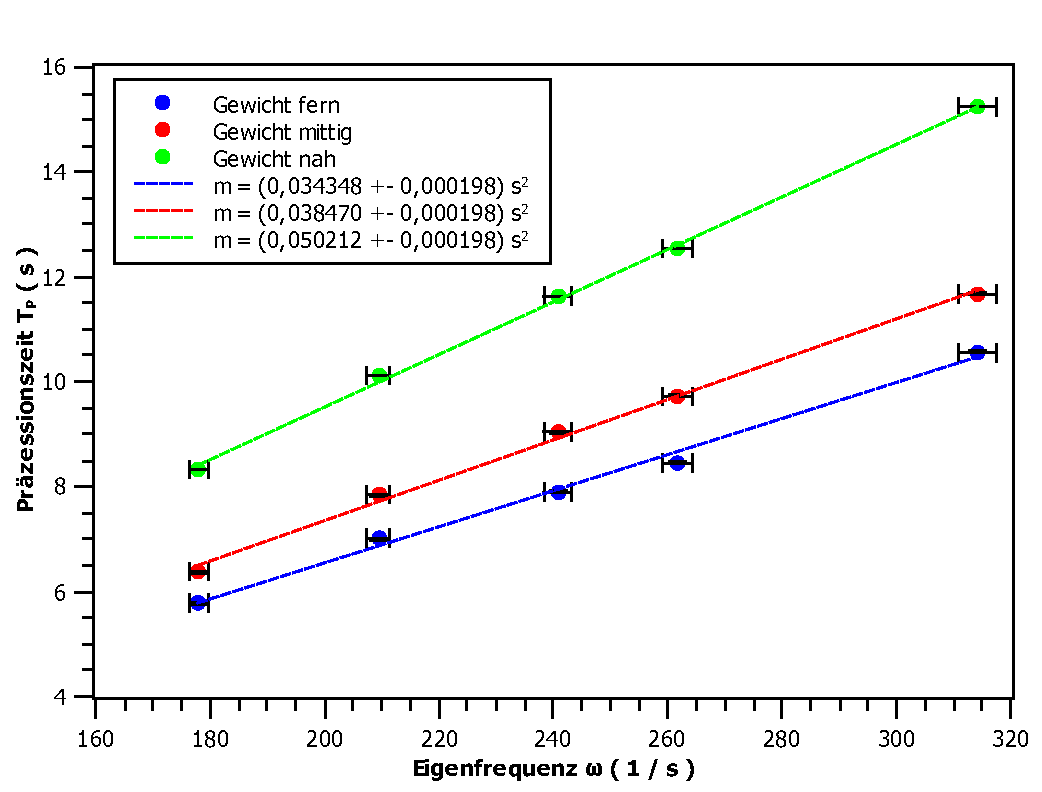
\includegraphics[width=\textwidth]{kreisel_wT_multi.pdf}
		\caption{Darstellung der Präzessionszeit gegen die Eigenfrequenz des Kreisel. Die drei unterschiedlichen Gewichtspositionen sind farblich gekennzeichnet.}
		\label{abb:Tw-multi}	
	\end{figure}
	Wie in Abb. \ref{abb:Tw-multi} zu erkennen ist, erhält man durch Linearisierung der Datenpunkte\footnote{Programm: SciDaVis; Algorithmus: kleinste Quadrate} für jede Gewichtsposition eine Steigung, im folgenden $m$ genannt.
	Dabei fällt auf, dass die Steigung größer ist, je näher das Gewicht an der Kugel ist.
	
	Nun werden die Punkte $(\frac{1}{m}, lF)$ in ein weiteres Diagramm gesetzt und ebenso linearisiert.
	\begin{figure}[ht]
		\centering
		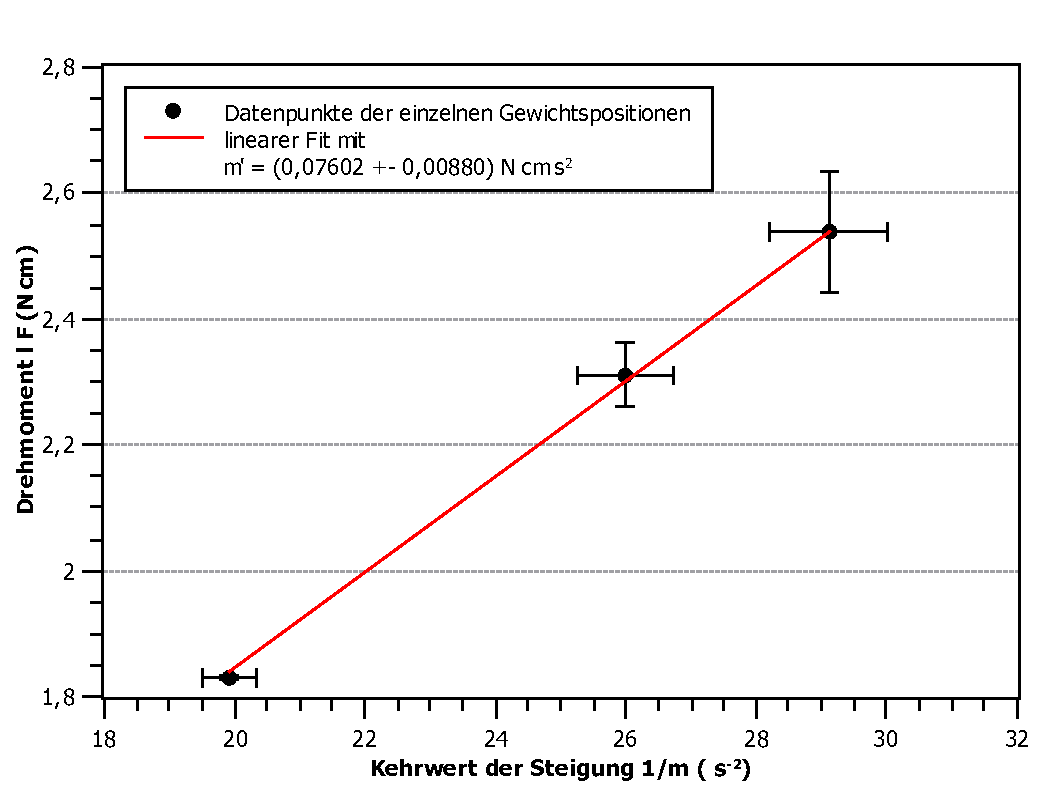
\includegraphics[width=\textwidth]{kreisel_gewichte.pdf}
		\caption{Darstellung und Linearisierung der drei Datensätze für unterschiedliche Gewichtspositionen. Es sei anzumerken, dass die Steigung die Einheit $\si{\newton\,\centi\meter\,\second\squared} = 10^5\cdot \si{g\,\centi\meter^2}$ hat.}
		\label{abb:gewichte}	
	\end{figure}
	Für die dort erhaltene Steigung gilt gerade eben $m' = \SI{0,07602 +- 0,00880}{\newton\,\centi\meter\,\second\squared} = 2\pi J$, bzw. umgestellt $J = \frac{m'}{2\pi}$.
	Nach beachten der Einheiten folgt:
	\begin{equation}
		J = \frac{m'}{2\pi} \approx \SI{1209,8 +- 140,1}{g\,\centi\meter\squared}
	\end{equation}
	

\subsection{Zusammenfassung}

Es wurde das Trägheitsmoment eines schweren, symmetrischen Kreisels auf zwei Arten ermittelt.
Zum einen wurde dieses durch die geometrische Form direkt berechnet.
Zum anderen konnte es durch die Präzession bei verschiedenen Positionen eines Zusatzgewichtes bestimmt werden.

Vergleicht man das graphisch ermittelte Trägheitsmoment mit dem geometrisch errechneten, so liegt letzteres in einem guten Vertrauensbereich.
Andersherum liegt aber der graphisch ermittelte Wert weit außerhalb des Vertrauensbereich des errechneten Wertes.


\subsection{Schlussfolgerung}

Die relative Unsicherheit des graphisch ermittelten Trägheitsmoment ist mit $10\%$ recht hoch.
Um weitere Übereinstimmungen zu erhalten, muss das Experiment ggf. noch einmal wiederholt werden, um einen schärferen graphischen Wert zu bekommen.
Dabei wäre es besonders wichtig, die Präzessionszeit über mehrere Perioden zu bestimmen und dabei die Eigenfrequenz des Kreisels konstant zu halten.
Das könnte z. B. durch eine längere Einpendelzeit vor der Messung eingebracht werden.
 
	
	%\section*{Literatur}
	%\printbibliography
	
	\newpage
	
	\section{Anhang} \label{Anhang}
		
	% Unsicherheitsrechnung & mehr
	
	\subsection{Unsicherheiten Fallrad}
	
	\begin{table}[ht]
		\centering
		\caption{einfache Unsicherheiten für die Werte bei der Berechnung für das Fallrad. Alle Unsicherheiten für Mittelwerte über fünf Werte (außer bei der Fadendicke, hier wurden sechs Werte aufgenommen). Da zur Vereinfachung der Messung Durchmesser und nicht Radien gemessen wurden, sind die Unsicherheiten in \ref{tab:Messwerte} um den Faktor 0.5 verschieden.}
		\begin{tabular}{l|l|l}
			{Unsicherheit $u$ der/des ...} & {Berechnung}  & {Ergebnis}\\
			\hline 
			{Stoppuhr} &  {$u_\text{Uhr}$ = $\frac{\SI{0,01}{\second}}{2\sqrt{3}}$} & {\SI{2,89}{\milli\second}} \\
			{Reaktionszeit} & {$u_\text{Reaktion} = \frac{\SI{0,1}{\second}}{2\sqrt{6}}$} & {\SI{20,4}{\milli\second}} \\
			{Zeitmessung} & {$u_\text{Zeit} = \sqrt{\left( u_\text{Uhr}\right) ^2+\left( u_\text{Reaktion}\right) ^2}$} & {\SI{20,6}{\milli\second}} \\
			{gemittelten Zeitmessung} & {$u_\text{ZeitMitt} = \sqrt{5\cdot\left(u_\text{Zeit}\right) ^2}$} & {\SI{46,1}{\milli\second}} \\
			\hline 
			{Maßes} &  {$u_\text{Maß}$ = $\frac{\SI{1}{\mm}}{2\sqrt{3}}$} & {\SI{0,29}{\mm}} \\
			{Schiebelehre} &  {$u_\text{Schiebe}$ = $\frac{\SI{0,04}{\mm}}{2\sqrt{3}}$} & {\SI{0,012}{\mm}} \\
			{gemittelten Längenmessung} &  {$u_\text{LängeMitt} = \sqrt{5\cdot\left(u_\text{Schiebe}\right) ^2}$} & {\SI{0,026}{\mm}} \\
			{Fadendicke} &  {$u_\text{FadenDicke} = \sqrt{6\cdot\left(u_\text{Schiebe}\right) ^2}$} & {\SI{0,028}{\mm}} \\
			\hline
			{Waage} & {$u_\text{Waage} = \frac{\SI{0,01}{\g}}{2\sqrt{6}}$} & \SI{0,002}{\g}{}
		\end{tabular}
	\end{table}

	Für die Unsicherheit der Fallhöhe $h$ wird die des Maßes $u_\text{Maß}$ und für die Fallzeit die Unsicherheit der gemittelten Zeitmessung $u_\text{ZeitMitt}$ verwendet. Für die Fallzeit zum Quadrat ergibt sich der folgende Zusammenhang:
	\begin{align*}
		u(t^2) = \sqrt{\left( \frac{\partial t^2}{\partial t}\cdot u_\text{ZeitMitt}\right) ^2}\\
			   = \sqrt{\left( 2 t\cdot u_\text{ZeitMitt}\right) ^2}.
	\end{align*}
	Ähnlich gilt für $\frac{h}{t^2}$:
	\begin{align*}
		u\left( \frac{h}{t^2}\right) = \sqrt{\left( \frac{\partial \frac{h}{t^2}}{\partial h}\cdot u_\text{Maß}\right) ^2 + \left( \frac{\partial \frac{h}{t^2}}{\partial t}\cdot u_\text{ZeitMitt}\right) ^2}\\
		= \sqrt{\left( \frac{1}{t^2}\cdot u_\text{Maß} \right) ^2 + \left(-2 \frac{h}{t^3}\cdot u_\text{ZeitMitt} \right) ^2}.
	\end{align*}
	Bei dem Trägheitsmoment sieht die Unsicherheitsberechnung komplizierter aus. Aus Gl. \ref{eq:Trägpar} folgt:
	\begin{align*}
		u(J_\text{parallel}) &= 
		\left[\left( \frac{\partial J_\text{parallel}}{\partial H}u(H)\right)^2  				
			+ \left( \frac{\partial J_\text{parallel}}{\partial \rho}u(\rho)\right)^2 \right.\\ 
			&\quad\left.+ \left( \frac{\partial J_\text{parallel}}{\partial R_a}u(R_a)\right)^2 
			+ \left( \frac{\partial J_\text{parallel}}{\partial R_i}u(R_i)\right)^2\right]^{\frac{1}{2}}.			 
	\end{align*}
	Beziehungsweise für das Trägheitsmoment für senkrecht zur Rotationsachse liegende Vollzylinder:
	\begin{align*}
		u(J_\text{senkrecht}) = \sqrt{\left( \frac{\partial J_\text{senkrecht}}{\partial H}u(H)\right)^2 				
			+ \left( \frac{\partial J_\text{senkrecht}}{\partial \rho}u(\rho)\right)^2 + 
			+ \left( \frac{\partial J_\text{senkrecht}}{\partial R}u(R)\right)^2}.			 
	\end{align*}
	$H$ ist bei beiden Gleichungen die Höhe bzw. Dicke des Zylinders. Für den Ring ist $u(H) =  u_\text{LängeMitt}$, für die Speichenzylinder ebenso, da deren Höhe $R_i$ entspricht und auch diese Größe fünf mal gemessen wurde. Für die Achse ist $u(H) =  u_\text{Schiebe}$. Zudem ist $u(R) = u_\text{Schiebe}$ für die Achse ($R_a = R, R_i = 0$ für diese), wie auch für die Speichenzylinder. Bei dem Ring ist $u(R_a) = u(R_i) = u(H) = u_\text{LängeMitt}$.
	Für alle Größen ist $u(\rho)$ gleich. Es setzt sich aus der Massenunsicherheit und der Volumenunsicherheit zusammen:
	\begin{align*}
		u(\rho) = \sqrt{\left( \frac{\partial \frac{m}{V}}{\partial m}u(m)\right)^2 + \left( \frac{\partial \frac{m}{V}}{\partial V}u(V)\right)^2} \\
			= \sqrt{\left(\frac{1}{V}u_\text{Waage}\right)^2 + \left(- \frac{m}{V^2}u(V)\right)^2}. 
	\end{align*}
	Dabei setzt sich $u(V)$ wie folgt zusammen aus V zusammen:
	\begin{align*}
		V &= H\cdot(\pi R_a^2 - \pi R_i^2) + 2(2\pi R_S\cdot 2 R_i) + 2\pi R_A\cdot L_A. \\		
		\Rightarrow u(V) &= \left[\left( \frac{\partial V}{\partial H}u(H)\right)^2 
			+ \left( \frac{\partial V}{\partial R_a}u(R_a)\right)^2 
			+ \left( \frac{\partial V}{\partial R_i}u(R_i)\right)^2 \right.\\ 
			&\quad\left.+ \left( \frac{\partial V}{\partial R_S}u(R_S)\right)^2 
			+ \left( \frac{\partial V}{\partial R_A}u(R_A)\right)^2 
			+ \left( \frac{\partial V}{\partial L_A}u(L_A)\right)^2\right]^{\frac{1}{2}} \\		
		&= \left[\left( (\pi R_a^2 - \pi R_i^2)u(H)\right)^2 
			+ \left( (2\pi H R_a)u(R_a)\right)^2 
			+ \left( (-2\pi H R_i+8\pi R_S)u(R_i)\right)^2 \right.\\ 
			&\quad\left.+ \left( (8\pi R_i)u(R_S)\right)^2 
			+ \left( (2\pi)u(R_A)\right)^2 
			+ \left( (1)u(L_A)\right)^2\right]^{\frac{1}{2}}		
	\end{align*}
	Dabei sind $u(H)=u(R_a)=u(r_i)=u_\text{LängeMitt}$ und $u(R_S)=u(R_A)=u(L_A)=u_\text{Schiebe}$.
	So ergeben sich für die drei verschiedenen Teile folgende Unsicherheiten für die Trägheitsmomente:
	\begin{align*}
	u(J_\text{Ring}) &= 
	\left[\left( (\frac{1}{2}\pi\rho (R_a^4 - R_i^4))u_\text{LängeMitt}\right)^2  				
		+ \left( (\frac{1}{2}\pi H (R_a^4 - R_i^4))u(\rho)\right)^2 \right.\\ 
		&\quad\left.+ \left( (2\pi H \rho R_a^3)u_\text{LängeMitt}\right)^2
		+ \left( (2\pi H \rho R_i^3)u_\text{LängeMitt}\right)^2\right]^{\frac{1}{2}}\\
	u(J_\text{Achse}) &= 
	\left[\left( (\frac{1}{2}\pi\rho R_S^4)u_\text{Schiebe}\right)^2  				
		+ \left( (\frac{1}{2}\pi L_A R_S^4)u(\rho)\right)^2  
		+ \left( (2\pi L_A \rho R_S^3)u_\text{Schiebe}\right)^2\right]^{\frac{1}{2}}\\
	u(J_\text{Speiche}) &= 
	\left[\left( (\frac{1}{4}\pi\rho R_i^2 R_S^2+\frac{1}{4}\pi\rho R_S^4)u_\text{LängeMitt}\right)^2  				
		+ \left( (\frac{1}{12}\pi R_i^3 R_S^2 + \frac{1}{4}\pi R_i R_S^4)u(\rho)\right)^2\right. \\ 
		&\quad\left.+ \left( (\frac{1}{6}\pi \rho R_i^3 R_S + \pi \rho R_i R_S^3)u_\text{LängeMitt}\right)^2\right]^{\frac{1}{2}}.	  
	\end{align*}
	Und somit schließlich für $J_S$:
	\begin{equation*}
		u(J_S)= \sqrt{u(J_\text{Ring})^2 + u(J_\text{Achse})^2 + u(J_\text{Speiche})^2}.
	\end{equation*}
	Für die Unsicherheit des Abrollradius' ergibt sich:
	\begin{align*}
		u(R) = \sqrt{\left( \frac{\partial R}{\partial J_S}u(J_S)\right)^2 + \left(\frac{\partial R}{\partial g^{*}}u(g^{*})\right) ^2} \\
		= \sqrt{\left( \frac{1}{2\sqrt{J_S g^{*} m(g-g^{*})}}u(J_S)\right)^2 + \left(\frac{1}{2\sqrt{J_S g^{*} m(g-g^{*})}}+\frac{m\sqrt{J_S g^{*}}}{2\sqrt{m(g-g^{*})}^3} u(g^{*})\right) ^2}.
	\end{align*}
	
	\subsection{Unsicherheiten für Kreisel}
	
	
	\begin{equation}
	\label{eq:unc_t}
	u(t) = \sqrt{u(t_R)^2 + u(t_D)^2} \approx \SI{0,020615}{\second}
	\end{equation}
	
	\begin{align}
	\label{eq:unc_traeg}
	u(J) = u(J_2) &= \frac{2}{5} \sqrt{\left( \pdv{m_k r_k^2}{m_k} u(m_k)\right) ^2 + \left( \pdv{m_k r_k^2}{r_k} u(r_k)\right) ^2}\\
	&= \frac{2}{5} \sqrt{(r_k^2 u(m_k))^2 + (2r_k m_k u(r_k))^2} \approx \SI{15,010472}{g\,\centi\meter\squared}
	\end{align}
	
	\begin{equation}
	\label{eq:unc_length}
	u(l) = \sqrt{u(L)^2 + u(r_k)^2 + u(h)^2} \approx \SI{0,015215}{\centi\meter}
	\end{equation}
	
	\begin{equation}
	\label{eq:unc_traeg2}
	u(J) = \frac{1}{2\pi} \pdv{m'}{m'} u(m') = \frac{u(m')}{2\pi}
	\end{equation}
	
\section*{Literatur}
	
	[1] Abb. \ref{fig:FallradSkizze} wurde der Einführung des Versuches aus dem LearnWeb entnommen.
	
\end{document} 